% 原文 pp.209–215（印刷 pp.1327–1333）
\section{Lecture 15：$\mathcal{N}=2$ 极小模型的 Landau–Ginzburg 描述与 Kähler 流形的量子上同调}

\begin{keytakeaways}
本讲前半部分系统整理了「某些 Landau--Ginzburg 模型的红外极限等于代数上可构造的 $\mathcal{N}=2$ 极小模型（minimal model）」这一断言的已有证据。物理图像是：超势的拟齐次性（quasi-homogeneity）给出一个可以延拓到超荷上的 $R$ 对称性，它的手征反常系数 $k$ 是拓扑不变量，可在紫外自由场论中精确算出，而它恰等于红外极限共形场论的中心荷 $\widehat{c}$。核心数学工具是 $\mathcal{N}=2$ 超共形代数的表示论、$\overline{Q}_+$（等价地 $\overline{D}_+$）上同调，以及椭圆亏格（elliptic genus）的路径积分与特征标两种算法。主要结论是 $\widehat{c}=\sum_j(1-2\alpha_j)$ 这一对各个手征超场逐项求和的公式，它把 Landau--Ginzburg 轨形、非线性 $\sigma$ 模型与加权射影空间中的 Calabi--Yau 超曲面串成同一条 UV--IR 链条。本讲末尾把这一图像接到加权射影空间与 Calabi--Yau 超曲面上，为后续的量子上同调（quantum cohomology）讨论作准备。
\end{keytakeaways}

% ===== 原文 p.209 =====

\subsection{Landau--Ginzburg 模型}
% 原文 §15.1：Landau-Ginzburg models

今天这讲前半部分的主题，是更详细地讨论一个已有断言所依据的已知证据：某些 Landau--Ginzburg 模型的红外（IR）极限，与那些代数上可构造的、被称为「极小模型」（minimal model）的共形场论（conformal field theory，CFT）等价。

先考虑最简单的 Landau--Ginzburg 模型：一个含单个手征超场（chiral superfield）$\Phi$ 的二维 $\mathcal{N}=2$ 理论，其拉氏量为
\[
  \mathcal{L}=\int d^2x\,d^4\theta\;\overline{\Phi}\Phi
  +\left(\int d^2x\,d\theta^+\,d\theta^-\,\Phi^k+{\rm c.c.}\right).
\]

我们在第 13 讲 §13.6.1 中的断言是：该模型在红外流向一个中心荷（central charge）为 $\widehat{c}=1-\frac{2}{k}$ 的共形场论。若此说成立，则它所流向的理论是代数可解的，因为中心荷 $\widehat{c}<1$ 的 $\mathcal{N}=2$ 超共形代数（superconformal algebra）的表示已有已知的分类。更确切地说，固定 $\widehat{c}=1-\frac{2}{k}$ 之后，该中心荷的代数的不可约表示 $\mathcal{H}_\alpha$ 只有有限多个（在同构意义下）。中心荷为 $\widehat{c}=1-\frac{2}{k}$ 的共形场论由其 Hilbert 空间完全确定，而这些 Hilbert 空间是由上述表示的张量积之和
\[
  \bigoplus_{\alpha,\beta}\left(\mathcal{H}_\alpha\otimes\overline{\mathcal{H}}_\beta\right)^{e_{\alpha\beta}}
\]
配以一个模不变（modular invariant）的特征标（character）构造出来的。这类组合有一个 $A$-$D$-$E$ 分类。其中最简单的模不变组合——也正是这里将会出现的那个——是对所有表示取无权对角和：
\[
  \bigoplus_{\alpha}\mathcal{H}_\alpha\otimes\overline{\mathcal{H}}_\alpha .
\]
（这对应于 $A$ 系列。）

更一般的 Landau--Ginzburg 模型含有若干个手征超场 $\Phi_1,\dots,\Phi_n$，以及一个拟齐次多项式（quasi-homogeneous polynomial）$W(\Phi_1,\dots,\Phi_n)$，它充当理论的超势（superpotential）。我们应当假定该多项式是横截的（transverse），

\noindent\textit{（本讲笔记整理者：John Morgan 与 David Morrison。）}

% ===== 原文 p.210 =====

其含义是 $W=dW=0$ 只在原点成立；而拟齐次性条件则可以表述为：存在正有理数 $\alpha_j$，使得
\[
  W=\sum_j\alpha_j\Phi_j\frac{\partial W}{\partial\Phi_j}.
\]

拉氏量可以写为
\[
  \mathcal{L}=\int d^2x\,d^4\theta\;\overline{\Phi}_j\Phi_j
  +\left(\int d^2x\,d\theta^+\,d\theta^-\,W(\Phi_j)+{\rm c.c.}\right).
\]

直观上，拟齐次性之所以重要，是因为它使得其中一个 $R$ 对称性（$R$-symmetry）有可能延拓为
\[
  \theta^+\to e^{i\varepsilon}\theta^+,\qquad \theta^-\to\theta^-,
\]
并作用在手征场上为 $\Phi_j\to e^{i\varepsilon\alpha_j}\Phi_j$，从而使超势按 $W\to e^{i\varepsilon}W$ 变换，拉氏量因而保持不变。如果我们假定这一微观的 $R$ 对称性在红外成为极限共形场论的左移 $R$ 对称性，那么我们就能借助算子乘积展开（operator product expansion，OPE）算出该极限理论的中心荷 $\widehat{c}$。

具体做法如下。回想在第 13 讲中我们遇到过一个常数 $k$，它度量的是：若试图把 $R$ 对称性 $J_L$ 规范化（gauging），会出现多大的反常（anomaly）。这个常数在算子乘积展开中表现为
\[
  J_L(x)J_L(x')=\frac{k}{(x^--x'^-)^2}+\cdots .
\]

把 $k$ 解释为规范化的阻碍，就立刻可以看出它是一个拓扑不变量，因而可以在任何标度下可靠地测量或计算。特别地，它可以在紫外（UV）计算，而在紫外超势无关紧要。（这样，规范化的阻碍是由一个指标问题（index problem）算出来的，无论我们所处的 Riemann 面是大是小都成立；我们可以把它取得足够小，以致超势完全无关。）另一方面，如果 $J_L$ 正是极限 $\mathcal{N}=2$ 超共形场论中出现的那同一个 $R$ 对称性，那么超共形代数的算子乘积展开就断言
\[
  J_L(x)J_L(x')=\frac{\widehat{c}}{(x^--x'^-)^2}+\cdots ,
\]
其中 $\widehat{c}$ 是 $\mathcal{N}=2$ 代数中的中心荷。于是 $k=\widehat{c}$，我们便可以通过在紫外做计算来测出红外的中心荷。

要在紫外计算 $k$，就把各个场当作自由场。规范化的阻碍来自这样一个事实：在自由的超多重态里，$R$ 对称性就是费米子的手征对称性。按照第 6 讲 §6.2 的方法，我们有 $k=\sum b_i^2-\sum c_i^2$，其中 $b_i$ 与 $c_i$ 分别是左手征费米子与右手征费米子的 $R$ 荷。在我们的问题里，$b_i=-1+\alpha_i$、$c_i=\alpha_i$，于是得到 $k=\sum_i(1-2\alpha_i)$。假定红外流向一个 $\mathcal{N}=2$ 理论、且其中出现同一个 $R$ 对称性，就有 $k=\widehat{c}$，从而 $\widehat{c}=\sum_j(1-2\alpha_j)$。注意：在单个场、$W(\Phi)=\Phi^k$ 的情形，必须有 $\alpha=1/k$，于是我们得到所期望的结果 $\widehat{c}=1-2/k$。

% [Tutor Note: 这一步是全讲最容易出错的地方，有两处要当心。其一，$k=\sum b_i^2-\sum c_i^2$ 中的 $b_i,c_i$ 是第 6 讲 §6.2 意义下左、右手征费米子的 $R$ 荷，而同一个手征超场 $\Phi_j$ 的两个费米子分量的荷相差 $1$（差的那个 $1$ 来自 $\int d^2\theta$ 测度、也就是超势的量纲），所以才会有 $b_i=-1+\alpha_i$ 而不是 $b_i=\alpha_i$；一旦漏掉这个 $-1$，就得到 $k=\sum\bigl(\alpha_i^2-\alpha_i^2\bigr)=0$，即"没有反常"，这与 $\widehat{c}=1-2/k$ 直接冲突。其二，是荷的平方差 $b_i^2-c_i^2$ 而不是差的平方 $(b_i-c_i)^2$：反常是荷平方之差的和，误写成一次差会把 $\alpha_i$ 的二阶项全部丢掉。最后，$\alpha=1/k$ 的来历作者没有写：把 $W=\Phi^k$ 代入拟齐次性条件得 $W=\alpha\Phi\,\partial_\Phi W=\alpha k\,\Phi^k$，故 $\alpha k=1$。]

我们现在要给出一个更精细的论证来支持这一等价性，它将揭示（极限）共形场论更多的结构。

% ===== 原文 p.211 =====

回想 $\mathcal{N}=2$ 代数的结构：
\[
  \{Q_\pm,\overline{Q}_\pm\}=P_\pm,\qquad \{Q_\pm,Q_\pm\}=0 .
\]
我们有 $\overline{Q}_+^2=0$，因此可以考察 $\overline{Q}_+$ 的上同调（cohomology），也就是考察那些满足 $\{\overline{Q}_+,\mathcal{O}\}=0$ 的局部算符 $\mathcal{O}=\mathcal{O}(x)$。于是
\[
  \partial_+\mathcal{O}=[\{Q_+,\overline{Q}_+\},\mathcal{O}]
  =[\overline{Q}_+,\{Q_+,\mathcal{O}\}],
\]
也就是说，用欧氏语言（把 $(x^+,x^-)$ 与 $(z,\overline{z})$ 等同起来），$\mathcal{O}(x)$ 在 $\overline{Q}_+$ 上同调中的类是全纯地变化的。

取两个这样的算符，用全纯语言写为
\[
  \mathcal{O}(z)\mathcal{O}'(z')=\sum_k f_k(z-z')\mathcal{O}_k(z')
  +\{\overline{Q}_+,\cdots\},
\]
其中 $f_k$ 是全纯函数。由这个公式可以看出，$\overline{Q}_+$ 上同调具有共形场论的一般结构，其中的算符是「纯左移的」，即它们全纯地变化。

一个重要注记是：$\overline{Q}_+$ 上同调在 Weyl 重标度（Weyl rescaling）下不变，因而它只依赖 Riemann 面的复结构（complex structure），而与度规无关。要看出这一不变性，我们必须证明 $T_{z\overline{z}}$ 是 $\overline{Q}_+$-恰当的（$\overline{Q}_+$-exact）。一个自然的证法是修改关于标度不变性的通常定义：利用多项式的拟齐次性，使得超势项在修改后的标度变换下保持不变。于是作用量中的动能项就不再标度不变，但动能项的改变量具有 $\int d^4\theta(\cdots)$ 的形式（因为动能项本身就有这一性质），从而是 $\overline{Q}_+$-恰当的。

% [Tutor Note: 作者说"一个自然的证法是修改标度不变性的定义"，这句话背后压掉了两小步。(1) 修改后的标度变换之所以能保住超势项，正是因为拟齐次性：给 $\Phi_j$ 赋权 $\alpha_j$、给 $\theta^+$ 赋权 $\frac12$、给 $\theta^-$ 赋权 $0$，$\int d^2\theta\,W$ 的总权才为零；若没有拟齐次性，$W$ 项单独就会被标度变换破坏，"修改定义"根本无从谈起。(2) 得到动能项的变分形如 $\int d^4\theta(\cdots)$ 之后，还要说明这类项在 $\overline{Q}_+$ 上同调中为零——用的正是本页上面那个恒等式：对 $\overline{Q}_+$-闭的算符，$\partial_+$ 作用后等于 $[\overline{Q}_+,\{Q_+,\cdot\}]$，自动落在 $\overline{Q}_+$ 的像里。所以"自然的证法"实质上是：用改进后的（无迹）能动张量把 $T_{z\overline{z}}$ 写成某个局部算符的全导数，再用 $\partial_+\mathcal{O}=[\overline{Q}_+,\{Q_+,\mathcal{O}\}]$ 收尾。]


以上我们用 $\overline{Q}_+$ 上同调来表述，是为了能涵盖非常一般的 $\mathcal{N}=2$ 理论。然而，只要理论有超空间实现（我们正在研究的 Landau--Ginzburg 理论正是如此），更方便的做法就是研究 $\overline{D}_+$ 上同调而非 $\overline{Q}_+$ 上同调，其中
\[
  \overline{D}_+=e^{-\theta^+\overline{\theta}^+\partial_+}\,
  \overline{Q}_+\,e^{\theta^+\overline{\theta}^+\partial_+},
\]
于是 $\overline{D}_+$ 上同调与 $\overline{Q}_+$ 上同调自然同构。

在我们的 Landau--Ginzburg 理论中，运动方程为
\[
  2\overline{D}_+\overline{D}_-\Phi^j=\frac{\partial W}{\partial\Phi^j}.
\]
考虑算符
\[
  \mathcal{T}=\sum_j\left(
  \left(\frac{1-\alpha_j}{2}\right)D_-\Phi^j\;\overline{D}_-\,\overline{\Phi}_j
  -i\alpha_j\,\overline{\Phi}_j\,\partial_-\Phi_j
  \right);
\]
则 $\overline{D}_+\mathcal{T}=0$，于是它定义了一个 $\overline{D}_+$ 上同调类。\footnote{此处本应担心反常，但实际上「$\overline{D}_+\mathcal{T}=0$」这一陈述并没有量子反常；不过在带 $(0,2)$ 超对称的二维模型中，一些颇为相似的陈述确实存在这类反常。参见 E.~Silverstein 与 E.~Witten, ``Global $U(1)$ $R$ Symmetry And Conformal Invariance Of $(0,2)$ Models,'' Phys.\ Lett.\ \textbf{B328} (1994) 307.}

% [Tutor Note: 这个 $\mathcal{T}$ 的指标写法在原书里并不统一，抄写时极易出错：第一项是 $D_-\Phi^j\,\overline{D}_-\,\overline{\Phi}_j$，前一个因子取上标 $j$、后一个取下标 $j$；而末项写成 $-i\alpha_j\overline{\Phi}_j\partial_-\Phi_j$ 时两个都取下标；到了 p.215 的 Kähler 项又写成 $\overline{\Phi}^j\Phi^j$（两个都取上标）。由于 $\Phi_j$ 与 $\overline{\Phi}_j$ 互为复共轭、$\alpha_j$ 为实数，这些写法在数值上等价，但若按"上下标必须成对缩并"的规则去读，会误以为原式有笔误。另外运动方程写成 $2\overline{D}_+\overline{D}_-\Phi^j=\partial W/\partial\Phi^j$，那个因子 $2$ 是约定相关的（取决于 $\overline{D}_\pm$ 的归一化，以及 Kähler 势取 $\overline{\Phi}\Phi$ 还是 $\frac12\overline{\Phi}\Phi$）；要核对 $\mathcal{T}$ 的两个系数 $(1-\alpha_j)/2$ 与 $i\alpha_j$ 是否配对正确，最可靠的办法就是按本页给出的运动方程把 $\overline{D}_+\mathcal{T}$ 实算一遍，并注意 $\overline{D}_+$ 只作用在含 $\overline{\theta}^+$ 的因子上。]

在自由理论中，取 $W=0$，$\mathcal{T}$ 是一个维数为 $(1,0)$ 的算符。如果我们面对的是超共形理论，就能把它写成
\[
  \mathcal{T}=J+\theta^-G+\overline{\theta}^-\,\overline{G}
  +\theta^-\overline{\theta}^-\,T .
\]

% ===== 原文 p.212 =====

如果我们确实在极限处得到一个 $\mathcal{N}=2$ 共形场论，那就应当期望有如下形式的 OPE：
\[
  \mathcal{T}(x)\mathcal{T}(y)=\frac{\widehat{c}}{(x-y)^2}
  +\frac{\mathcal{T}}{(x-y)}+\text{关于 }\mathcal{O}\text{ 全纯的项}.
\]
在自由场论中我们可以验证这一结构：第一项来自形如下图的一个图，其中两个算符之间交换了两条传播子：

\begin{figure}[htbp]
  \centering
  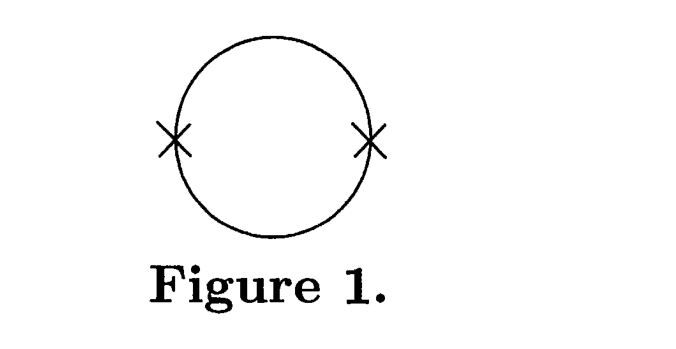
\includegraphics[width=0.30\textwidth]{figs/fig_p212_1.png}
  \caption{第一项所对应的图形：两个算符之间交换两条传播子，构成一个闭合的圈（单圈自收缩图），给出 $1/(x-y)^2$ 型的接触项，其系数即中心荷 $\widehat{c}$。（原文 Figure 1，p.212）}
  \label{fig:p212-1}
\end{figure}

\noindent 而第二项则来自形如下图的一个图，其中只交换了一条传播子：

\begin{figure}[htbp]
  \centering
  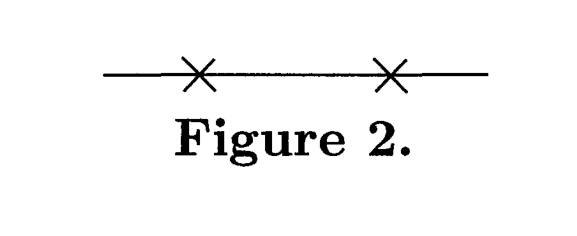
\includegraphics[width=0.26\textwidth]{figs/fig_p212_2.png}
  \caption{第二项所对应的图形：两个算符之间只交换一条传播子，给出 $1/(x-y)$ 型的项，其算符系数即 $\mathcal{T}$ 本身。（原文 Figure 2，p.212）}
  \label{fig:p212-2}
\end{figure}

\noindent 其中只交换了一条传播子。

请注意，在算子乘积展开中计算这些项时，我们可以令 $W=0$，因为超势项太软（too soft，即可超重整化），不会对这些奇异性有贡献。这样做完之后，不同的超场彼此解耦，于是 $\widehat{c}$ 的计算就是各个超场贡献之和。由此立刻得到一个结论：$\widehat{c}$ 对 $\alpha_j$ 是可加的，即 $\widehat{c}=\sum_j f(\alpha_j)$，其中 $f$ 是某个函数。具体计算给出 $f(\alpha)=1-2\alpha$，与我们第一种做法一致。

% [Tutor Note: "超势太软"这句话在二维要按量纲来读：二维中 $\int d^2\theta\,W$ 无量纲、而 $d^2\theta$ 的量纲为 $1$，故 $[W]=1$；于是超势只能产生可去的小动量行为，无法生成 $1/(x-y)^2$ 这种短距离奇异性，因此在算 OPE 奇异项时尽可令 $W=0$。这一点是关键：正因如此不同超场才解耦，$\widehat{c}$ 才对 $\alpha_j$ 可加，$\widehat{c}=\sum_j f(\alpha_j)$ 才成立。顺带提醒，此处加的是 $\widehat{c}=c/3$：若误用 $c$，可加性形式上仍成立但数值差三倍，在 $W=\Phi^k$ 时就会把 $c=3(1-2/k)$ 与 $c=1-2/k$ 混为一谈。至于这两个图，要注意 Figure 1 是"算符—算符"之间的单圈自收缩（两条传播子），不要读成双圈图；Figure 2 才是单传播子交换。]

总之，即使在我们这个微观拉氏量里，也能看到一个算符 $\mathcal{T}$，它在 $\overline{D}_+$ 上同调这一层面上满足 $\mathcal{N}=2$ 超共形代数。因此可以推测：该理论在红外流向一个共形场论，而其 $\overline{D}_+$ 上同调包含该超共形代数。

如果我们只有一个手征超场，从而 $\widehat{c}<1$，那么 $\mathcal{N}=2$ 代数在量子 Hilbert 空间中的作用几乎是不可约的。因此应当期望 $\mathcal{T}$ 会生成 $\overline{Q}_+$ 上同调。对于 $\widehat{c}>1$，$\mathcal{N}=2$ 代数的作用方式远非不可约，要得到一个代数可解的模型就需要额外的生成元。至于某些 Landau--Ginzburg 模型是否真的存在这样的额外生成元，目前尚不清楚（除了超势为若干不同变量的函数之和这一显然情形之外）。

\subsection{椭圆亏格}
% 原文 §15.2：The elliptic genus

我们将通过椭圆亏格（elliptic genus）的计算，给出这些理论之间等价性的更多证据。我们在亏格 $1$ 的 Riemann 面上工作，其周期格由 $1$ 与 $\tau$ 张成。

\begin{figure}[htbp]
  \centering
  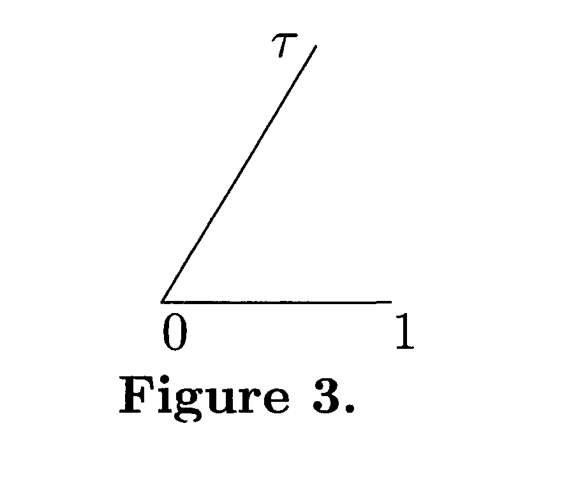
\includegraphics[width=0.34\textwidth]{figs/fig_p212_3.png}
  \caption{亏格 $1$ Riemann 面的周期格：由 $1$ 与 $\tau$ 张成，$\tau$ 取在上半平面。（原文 Figure 3，p.212）}
  \label{fig:p212-3}
\end{figure}

% ===== 原文 p.213 =====

我们令 $q=e^{2\pi i\tau}$，并计算
\[
  \mathrm{Tr}\;q^{(H-P)/2}\,\overline{q}^{(H+P)/2}(-1)^{F_R}.
\]

在环面的空间方向上，我们对左移与右移费米子都取周期边界条件。插入 $(-1)^{F_R}$ 意味着：右移费米子 $\psi_+,\overline{\psi}_+$ 在时间方向上也应当取周期边界条件，从而构成奇（odd）旋量结构（即在两个方向上都周期的那一种）；而左移费米子 $\psi_-,\overline{\psi}_-$ 在时间方向上应当是反周期的，因而它们是偶（even）旋量丛的截面。

\begin{figure}[htbp]
  \centering
  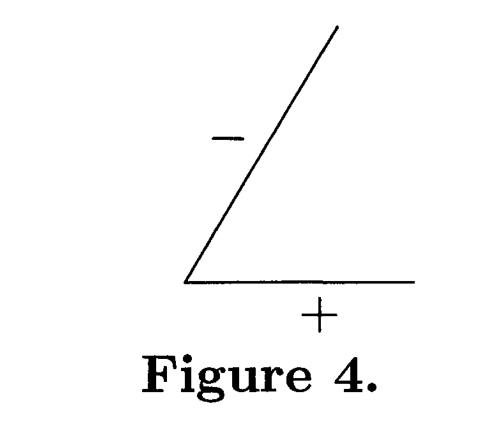
\includegraphics[width=0.26\textwidth]{figs/fig_p213_1.png}
  \caption{环面上两组费米子边界条件的示意：水平边标以「$+$」，斜边标以「$-$」，表示一组费米子在两个方向上都取周期（奇旋量结构）、另一组在时间方向取反周期（偶旋量结构）。（原文 Figure 4，p.213）}
  \label{fig:p213-1}
\end{figure}

% [Tutor Note: 自旋结构这句话最容易记反。按本文的 $\pm$ 约定，$\psi_+$ 是右移、$\psi_-$ 是左移；空间方向两者都取周期（环面上空间方向没有别的选择），时间方向则由 $(-1)^{F_R}$ 的插入决定：$\psi_+$ 在时间方向也周期（两方向皆周期 $=$ 奇旋量结构），$\psi_-$ 在时间方向反周期（偶旋量丛）。若把插入误写成 $(-1)^{F_L}$，两个 $\pm$ 的角色互换，所得函数会变成以 $\overline{q}$ 展开的那一个，与 p.215 的乘积公式对不上。一个现成的自洽性检验是：p.215 的最终结果只含 $q$、不含 $\overline{q}$，这正与 p.214 中"右移部分被 $(-1)^{F_R}$ 投影到基态、只剩 $1$ 或 $0$"相吻合。]

带这些边界条件的路径积分只需 $\mathcal{N}=1$ 超对称就能引入；而且正如我们去年秋天讨论过的，单在这一背景下它就已经相当有趣。它可以被解释为 $\mathcal{N}=1$ 理论右移超荷的指标（index）。

在 $\mathcal{N}=2$ 超对称的情形，故事更有意思，因为还有进一步丰富的余地：可以在迹中插入 $e^{i\gamma J_L}$，它与 $Q_+$ 和 $\overline{Q}_+$ 都对易，因而保持了「指标」这一解释。\footnote{我们对左 $R$ 流以及由它导出的守恒荷使用同一个符号 $J_L$。}我们考虑函数
\[
  F(q,\gamma)=\mathrm{Tr}\;q^{(H-P)/2}\,\overline{q}^{(H+P)/2}\,
  e^{i\gamma J_L}(-1)^{F_R}.
\]

为了用路径积分表示这个迹，我们按惯例把一个柱面的两端粘起来，构造出亏格 $1$ 的曲面（两端分别等同于初时刻与末时刻）。迹中的 $e^{i\gamma J_L}$ 因子是这样并入路径积分的：把初、末数据在粘接时乘以 $e^{i\gamma J_L}$；迹中其他因子也照此类推。

第一个观察是：量 $F(q,\gamma)$ 与理论中任何保持 $\mathcal{N}=2$ 结构的连续变化参数无关。这是因为它是若干项之和，而每一项都是某个算符的指标。出于同样的理由（或者因为理论能动张量的迹是 $\overline{Q}_+$-恰当的），$F(q,\gamma)$ 在环面度规的重标度下不变，因而只依赖复结构。

我们想在两个场合计算 $F(q,\gamma)$：(i) 在红外，对已知的代数构造模型作代数计算；(ii) 在紫外，直接对 Landau--Ginzburg 模型作计算。二者相比较，将为「Landau--Ginzburg 理论在红外确实流向极小模型」提供更多证据。

\subsubsection{红外中的代数计算}
% 原文 §15.2.1：Algebraic calculation in the IR

「极小模型」（在 $A$ 系列中，与这里所考虑的模型相关）的 Hilbert 空间形如 $\mathcal{H}=\bigoplus_\alpha\mathcal{H}_\alpha\otimes\overline{\mathcal{H}}_\alpha$，其中左移部分在 $\mathcal{H}_\alpha$ 中，右移部分在 $\overline{\mathcal{H}}_\alpha$ 中。（求和跑遍中心荷 $\widehat{c}=1-2/k$ 的 $\mathcal{N}=2$ 超共形代数在 Ramond 扇区的所有酉不可约表示，也就是

% ===== 原文 p.214 =====

在圆上取非束缚（non-bounding）旋量结构的那些表示。）因此，椭圆亏格可以写为
\[
  F(q,\gamma)=\sum_\alpha
  \left(\mathrm{Tr}_{\mathcal{H}_\alpha}\,q^{(H-P)/2}e^{i\gamma J_L}\right)
  \left(\mathrm{Tr}_{\overline{\mathcal{H}}_\alpha}\,
  \overline{q}^{(H+P)/2}(-1)^{F_R}\right).
\]

右移部分的贡献 $\mathrm{Tr}_{\overline{\mathcal{H}}_\alpha}\overline{q}^{(H+P)/2}(-1)^{F_R}$，当 $\overline{\mathcal{H}}_\alpha$ 的最高权满足 $H+P=0$ 时取值 $1$，否则取值 $0$。其效果是从这些不可约表示中挑出一个特定的子集。我们引入一个限制求和 $\sideset{}{'}\sum_\alpha$ 来表示对该子集求和。于是椭圆亏格可写为
\[
  F(q,\gamma)=\sideset{}{'}\sum_{\alpha}
  \mathrm{Tr}_{\mathcal{H}_\alpha}\,q^{(H-P)/2}e^{i\gamma J_L}.
\]

（请注意：荷 $J_L$ 的本征值一般不是整数。确切地说，量 $\exp(2\pi iJ_L)$ 与 $\mathcal{N}=2$ 代数对易，并且在每个表示中都是常数；这个常数依赖各个手征原初场的 $R$ 荷，而后者是有理数。因此 $F(q,\gamma)$ 关于 $\gamma$ 是周期的，但周期并不是 $2\pi$。）利用这个公式，$F(q,\gamma)$ 可以由 $\mathcal{N}=2$ 超共形代数的特征标公式算出。

% [Tutor Note: 括号里这段话是读特征标公式时的关键提醒，值得展开。$J_L$ 的本征值不是整数，是因为手征原初场带 $R$ 荷 $\alpha$，其 $J_L$ 荷被平移了 $\alpha$（谱流，spectral flow）；只有在 $\exp(2\pi iJ_L)$ 这一层面上平移才"看不见"。又因为 $\alpha$ 是有理数，$\exp(2\pi iJ_L)$ 在每个不可约表示中等于常数 $e^{2\pi i c_\alpha}$，$c_\alpha\in\mathbb{Q}$，所以把 $\gamma$ 平移 $2\pi$ 只是把每一项乘上这个常数，$F$ 的周期是 $2\pi$ 的某个有理倍数，而并不是 $2\pi$。做数值核对时若先验地假定 $F(q,\gamma+2\pi)=F(q,\gamma)$，就会得出"公式不自洽"的错误结论。]

\subsubsection{紫外中的直接计算}
% 原文 §15.2.2：Direct calculation in the UV

回到 Landau--Ginzburg 理论，我们可以试着在紫外直接计算。我们利用 $F(q,\gamma)$ 与环面面积无关这一事实，把面积取得非常小。粗略地说，在紫外相互作用可以忽略，我们应当能够取 $W=0$。唯一使这一点失效的原因，与大场的行为有关。作用量的玻色部分为
\[
  \int d\mu\,|d\phi|^2+\int d\mu\left|\frac{dW}{d\phi}\right|^2 .
\]

这里 $d\mu$ 是环面的 Riemann 测度。存在 $W$ 项时，作用量的唯一极小点是 $\phi=0$。如果我们把 $W$ 设为零，那么任何常值 $\phi$ 都使作用量取极小；即使在路径积分的首阶近似中，也必须对常值 $\phi$ 构成的空间积分，而一旦 $\phi$ 变得足够大，$W$ 项（只要它的系数不严格为零）就变得重要了。

于是结论是：只要 $\phi$ 是环面上的一个\emph{函数}，$W$ 项就不能被完全忽略。然而，如果 $\phi$ 不是函数，而是某个非平凡平坦丛的一个截面，那么即使 $W=0$，作用量中 $|d\phi|^2$ 那一部分也会有一个唯一的、非退化的极小点。在这种情形下，在环面面积趋于零的极限下把 $W$ 设为零就是顺理成章的。

在 $F(q,\gamma)$ 的路径积分计算中，对于一般的 $\gamma$，我们遇到的正是这种情形：$\phi$ 是一个非平凡平坦丛的截面。理由是 $J_L$ 作用在 $\phi$ 上为 $\delta\phi=\alpha\phi$。在用路径积分计算椭圆亏格时，$\phi$ 是环面上的一个场，它满足
\[
  \phi(P+\tau)=e^{i\gamma\alpha}\phi(P).
\]
（这里我们把环面视为复平面除以由 $1$ 与 $\tau$ 生成的格所得的商，$P$ 是复平面上的任一点。）因此 $\phi$ 是由这一粘接方式所规定的、环面上某个平坦丛的截面。若 $\gamma$ 是一般的，这个平坦丛就是非平凡的，而 $\phi=0$ 是作用量的一个孤立的、非退化的极小点，

% ===== 原文 p.215 =====

即使令 $W=0$ 也如此。这种非退化性使计算变得直截了当：$F(q,\gamma)$ 的计算就是令 $W=0$，并把 $F$ 表示成行列式之比。说明其中的细节会把我们带得太远，但结果是
\[
  F(q,\gamma)=e^{-i\gamma k\alpha/2}\cdot
  \frac{1-e^{i\gamma(k+1)\alpha}}{1-e^{i\gamma\alpha}}\cdot
  \prod_{n=1}^{\infty}
  \frac{\left(1-q^ne^{i\gamma(k+1)\alpha}\right)\left(1-q^ne^{-i\gamma(k+1)\alpha}\right)}
  {\left(1-q^ne^{i\gamma\alpha}\right)\left(1-q^ne^{-i\gamma\alpha}\right)} .
\]

把这个结果与红外中的代数计算相比较，就可以提取出 $\mathcal{N}=2$ 代数某些特征标的公式。这些公式可以独立地加以验证，从而有力地支持了「Landau--Ginzburg 理论在红外流向 $\mathcal{N}=2$ 极小模型」这一断言。

% [Tutor Note: 这个乘积公式可以做两个立即可做的检验。(1) 令 $\gamma\to0$：分子 $1-e^{i\gamma(k+1)\alpha}$ 与分母 $1-e^{i\gamma\alpha}$ 之比趋于 $k+1$，无穷乘积中每个 $n$ 的因子都趋于 $1$，故 $F(q,0)=k+1$；这应当等于该模型基态（Ramond 基态）的数目，而它正是 $W=\Phi^{k+2}$ 的临界点个数 $\partial W=(k+2)\Phi^{k+1}=0$。(2) 全式只依赖 $q=e^{2\pi i\tau}$ 而不依赖 $\overline{q}$，与椭圆亏格只依赖复结构、右移部分被投影掉这一点一致。把 $F(q,0)=k+1$ 与 $\widehat{c}=\sum_j(1-2\alpha_j)$ 联立，可反推出本式所用的归一化是 $\alpha=1/(k+2)$、$\widehat{c}=1-2/(k+2)$。要特别小心：这里的 $k$ 与 p.210 的 $k$ 并不是同一个量（那里 $k=\widehat{c}$ 是手征反常系数），原书复用同一字母而不加区分，是本讲最隐蔽的记号陷阱。]

\subsubsection{与 Calabi--Yau 模型的联系}
% 原文 §15.2.3：Connection to Calabi-Yau models

现在考虑这样一个 $U(1)$ 规范理论：手征超场 $\Phi_j$ 的荷为 $\alpha_j$，另有荷为 $-1$ 的场 $P$，并且 $\sum\alpha_j=1$。（我们不再假定所有 $\alpha_j$ 都相等，而且对 $U(1)$ 生成元所用的归一化也与第 13 讲不同。）把规范超多重态记为
\[
  \Sigma=\sigma+\cdots,
\]
设 $W(\Phi_1,\dots,\Phi_n)$ 是如上那样的横截、拟齐次多项式（即满足 $W=\sum_j\alpha_j\Phi_j\frac{\partial W}{\partial\Phi_j}$，且 $W=dW=0$ 只在原点成立），并考虑拉氏量
\[
  \begin{aligned}
  \mathcal{L}={}&\int d^2x\,d^4\theta\left(
  \frac{\overline{\Sigma}\Sigma}{4e^2}+\overline{\Phi}^j\Phi^j\right)
  +\left(\int d^2x\,d^2\theta\,PW(\Phi)+{\rm c.c.}\right)\\
  &+\left(\int d^2x\,d\theta^+\,d\theta^-\,t\Sigma+{\rm c.c.}\right),
  \end{aligned}
\]
其中 $t=\frac{\theta}{2\pi}-ir$。

多项式 $PW(\Phi)$ 是规范不变的，于是我们可以重复第 13 讲的讨论：当 $r\gg0$ 时，经典地得到加权射影空间（weighted projective space）$\mathbf{WCP}^{n-1}_{(\alpha_1,\dots,\alpha_n)}$ 中的 Calabi--Yau 超曲面 $\{W=0\}$（该超曲面可能从加权射影空间自身的奇点继承一些奇点）；当 $r\ll0$ 时，我们得到一个超势为 $W$ 的 Landau--Ginzburg 轨形（orbifold）。量子理论只在 $r=r_0$、$\theta=0$ 时才是奇异的。（$r_0$ 是一个按第 13 讲算出的常数。）在 Landau--Ginzburg 理论中计算中心荷给出
\[
  \widehat{c}=\sum_j(1-2\alpha_j);
\]
而在 $\sigma$ 模型中计算则给出 $\widehat{c}=\dim_{\mathbb{C}}X$，二者一致，因为 $\sum\alpha_j=1$。

\begin{figure}[htbp]
  \centering
  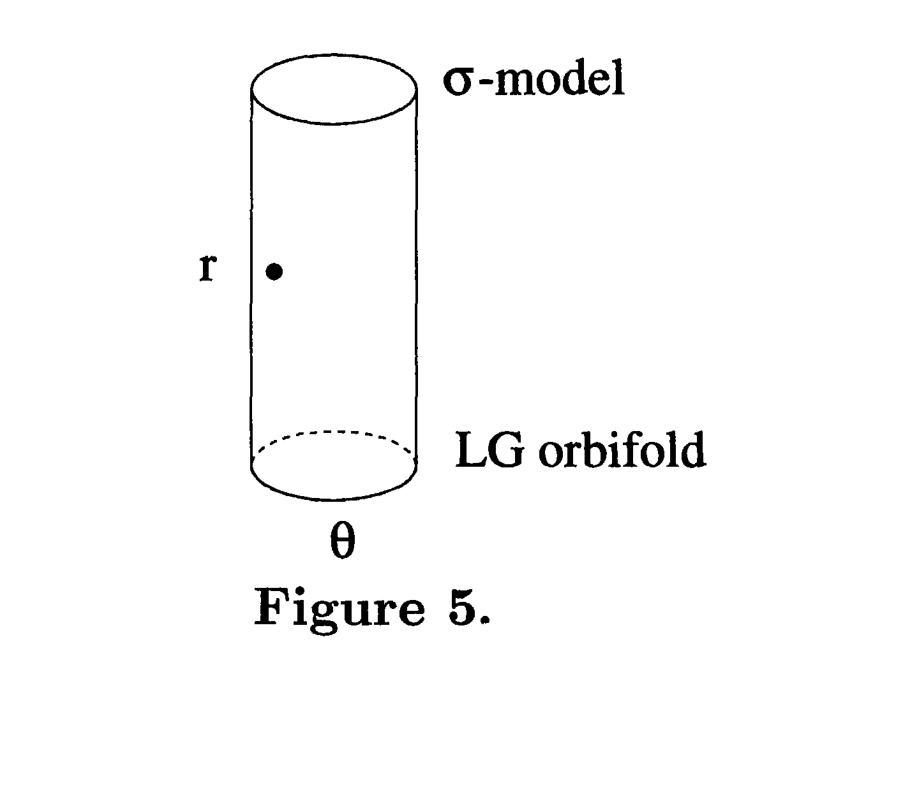
\includegraphics[width=0.40\textwidth]{figs/fig_p215_1.png}
  \caption{$r$--$\theta$ 柱面：竖直方向为 $r$，绕柱的圆周方向为 $\theta$。柱顶标注 $\sigma$-model（$r\gg0$ 的一端），柱底标注 LG orbifold（$r\ll0$ 的一端）；柱面上的黑点示意量子理论出现奇异的位置，对应 $r=r_0$、$\theta=0$。（原文 Figure 5，p.215）}
  \label{fig:p215-1}
\end{figure}
